\documentclass[11pt]{article}

\newcommand{\yourname}{Kevin Zhang}

\def\comments{0}

%format and packages

%\usepackage{algorithm, algorithmic}
\usepackage{tikz}
\usepackage{algpseudocode}
\usepackage{amsmath, amssymb, amsthm}
\usepackage{tcolorbox}
\usepackage{enumerate}
\usepackage{enumitem}
\usepackage{framed}
\usepackage{verbatim}
\usepackage[margin=1.0in]{geometry}
\usepackage{microtype}
\usepackage{kpfonts}
\usepackage{palatino}
	\DeclareMathAlphabet{\mathtt}{OT1}{cmtt}{m}{n}
	\SetMathAlphabet{\mathtt}{bold}{OT1}{cmtt}{bx}{n}
	\DeclareMathAlphabet{\mathsf}{OT1}{cmss}{m}{n}
	\SetMathAlphabet{\mathsf}{bold}{OT1}{cmss}{bx}{n}
	\renewcommand*\ttdefault{cmtt}
	\renewcommand*\sfdefault{cmss}
	\renewcommand{\baselinestretch}{1.06}

\usepackage[boxruled,vlined,nofillcomment]{algorithm2e}
	\SetKwProg{Fn}{Function}{\string:}{}
	\SetKwFor{While}{While}{}{}
	\SetKwFor{For}{For}{}{}
	\SetKwIF{If}{ElseIf}{Else}{If}{:}{ElseIf}{Else}{:}
	\SetKw{Return}{Return}
	

%enclosure macros
\newcommand{\paren}[1]{\ensuremath{\left( {#1} \right)}}
\newcommand{\bracket}[1]{\ensuremath{\left\{ {#1} \right\}}}
\renewcommand{\sb}[1]{\ensuremath{\left[ {#1} \right\]}}
\newcommand{\ab}[1]{\ensuremath{\left\langle {#1} \right\rangle}}

%probability macros
\newcommand{\ex}[2]{{\ifx&#1& \mathbb{E} \else \underset{#1}{\mathbb{E}} \fi \left[#2\right]}}
\newcommand{\pr}[2]{{\ifx&#1& \mathbb{P} \else \underset{#1}{\mathbb{P}} \fi \left[#2\right]}}
\newcommand{\var}[2]{{\ifx&#1& \mathrm{Var} \else \underset{#1}{\mathrm{Var}} \fi \left[#2\right]}}

%useful CS macros
\newcommand{\poly}{\mathrm{poly}}
\newcommand{\polylog}{\mathrm{polylog}}
\newcommand{\zo}{\{0,1\}}
\newcommand{\pmo}{\{\pm1\}}
\newcommand{\getsr}{\gets_{\mbox{\tiny R}}}
\newcommand{\card}[1]{\left| #1 \right|}
\newcommand{\set}[1]{\left\{#1\right\}}
\newcommand{\negl}{\mathrm{negl}}
\newcommand{\eps}{\varepsilon}
\DeclareMathOperator*{\argmin}{arg\,min}
\DeclareMathOperator*{\argmax}{arg\,max}
\newcommand{\eqand}{\qquad \textrm{and} \qquad}
\newcommand{\ind}[1]{\mathbb{I}\{#1\}}
\newcommand{\sslash}{\ensuremath{\mathbin{/\mkern-3mu/}}}

%mathbb
\newcommand{\N}{\mathbb{N}}
\newcommand{\R}{\mathbb{R}}
\newcommand{\Z}{\mathbb{Z}}
%mathcal
\newcommand{\cA}{\mathcal{A}}
\newcommand{\cB}{\mathcal{B}}
\newcommand{\cC}{\mathcal{C}}
\newcommand{\cD}{\mathcal{D}}
\newcommand{\cE}{\mathcal{E}}
\newcommand{\cF}{\mathcal{F}}
\newcommand{\cL}{\mathcal{L}}
\newcommand{\cM}{\mathcal{M}}
\newcommand{\cO}{\mathcal{O}}
\newcommand{\cP}{\mathcal{P}}
\newcommand{\cQ}{\mathcal{Q}}
\newcommand{\cR}{\mathcal{R}}
\newcommand{\cS}{\mathcal{S}}
\newcommand{\cU}{\mathcal{U}}
\newcommand{\cV}{\mathcal{V}}
\newcommand{\cW}{\mathcal{W}}
\newcommand{\cX}{\mathcal{X}}
\newcommand{\cY}{\mathcal{Y}}
\newcommand{\cZ}{\mathcal{Z}}

%theorem macros
\newtheorem{thm}{Theorem}
\newtheorem{lem}[thm]{Lemma}
\newtheorem{fact}[thm]{Fact}
\newtheorem{clm}[thm]{Claim}
\newtheorem{rem}[thm]{Remark}
\newtheorem{coro}[thm]{Corollary}
\newtheorem{prop}[thm]{Proposition}
\newtheorem{conj}[thm]{Conjecture}

\theoremstyle{definition}
\newtheorem{defn}[thm]{Definition}
\newtheoremstyle{case}{}{}{}{}{}{:}{ }{}
\theoremstyle{case}
\newtheorem{case}{Case}

\theoremstyle{theorem}
\newtheorem{prob}{Problem}
\newtheorem{sol}{Solution}

\begin{document}
{\large
\noindent Name: \yourname}

\vspace{15pt}

\begin{prob}\end{prob}

\begin{enumerate}[label=(\alph*)]
\item
Given a function $f: X \rightarrow Y$ where $X$ and $Y$ are finite sets, and $|X| = |Y|$. 
Suppose that $f$ is injective. This means for every element $y \in Y$, there is at most one arrow
pointing in. But, $f$ is a function, which means for every unique $x \in X$, there must be an arrow 
going from $x$ to $y$. Since no $y$ can have more than one arrow pointing in, and $|X| = |Y|$, 
then the number of arrows pointing in must be exactly 1 for every $y$. This implies that $f$ is bijective,
which then implies that $f$ must also be surjective as well.

\item
Given a fucntion $f: X \rightarrow Y$ where $X$ and $Y$ are finite sets, and $|X| = |Y|$.
Suppose that $f$ is surjective. This means that for every element $y \in Y$, there is at least
one arrow pointing in. But $f$ is a function, which means there cannot be more 
than one arrow pointing out for every $x \in X$. Since $|X| = |Y|$, it is not possible for there to
be any $y$ with more than one arrow pointing in, which means there is exactly 1 arrow pointing in for
every $y$. This implies that $f$ is bijective, which then implies that $f$ must also be injective as well.

\end{enumerate}


\begin{prob}\end{prob}

\begin{enumerate}[label=(\alph*)]
\item 
A function that produces every $n^{th}$ prime number. Some numbers are not prime, and will have no arrows 
pointing into them, making the function not surjective by default.

\item
A function that produces the smallest factor of $n$. Multiple numbers will have the same smallest factor (eg. 2), 
making this surjective, but not injective.

\end{enumerate}

\begin{prob}\end{prob}

\begin{tabular}{|c|c|c|c|c|c|c|}
$3^6$ & $3^5$ & $3^4$ & $3^3$ & $3^2$ & $3^1$ & $3^0$ \\
b & c & a & c & b & a & b
\end{tabular}

\vspace{15px}

In b-adic ordering, $a = 1$, $b = 2$, and $c = 3$, so the total would be 
$$(3^6 \times 2) + (3^5 \times 3) + (3^4 \times 1) + (3^3 \times 3) + (3^2 \times 2) + (3^1 \times 1) + (3^0 \times 2) = \textbf{2372}$$

\begin{prob}\end{prob}

Number 909 can be broken down as follows:
\begin{align*}
909 &= 3 \times 302 + \textbf{3} \\
302 &= 3 \times 100 + \textbf{2} \\
100 &= 3 \times 33 + \textbf{1} \\
33  &= 3 \times 10 + \textbf{3} \\
10  &= 3 \times 3 + \textbf{1} \\
3   &= 3 \times 0 + \textbf{3}
\end{align*}

With $a = 1$, $b = 2$, and $c = 3$, the string would be $\textbf{cbacac}$. \\

\newpage

\begin{prob}\end{prob}

If we assign a bit vector to each of the results from $f$, we would get:
\begin{align*}
f(a) &= \{a, b\} &\rightarrow 1 \space 1 \space 0 \space 0 \space 0 \\
f(b) &= \{c, d, e\} &\rightarrow 0 \space 0 \space 1 \space 1 \space 1 \\
f(c) &= \{b, c\} &\rightarrow 0 \space 1 \space 1 \space 0 \space 0 \\
f(d) &= \varnothing &\rightarrow 0 \space 0 \space 0 \space 0 \space 0 \\
f(e) &= \{a, c, d\} &\rightarrow 1 \space 0 \space 1 \space 1 \space 0
\end{align*}

We can then take the flipped diagonal, and we get the bit-vector $0 \space 1 \space 0 \space 1 \space 1$, which corresponds
to the set $\{b, d, e\}$.

\begin{prob}\end{prob}

For the sets in the sequence $S_0, S_1, S_2, ...$ of subsets of $\N$, we are only concerned
with the even numbers in each set (since $S$ can contain only evens), so we can form the diagram as such: \\

\begin{tabular}{|c|c|c|c|c|c|}

$\space$ & $0$ & $2$ & $4$ & $6$ & ... \\

\hline

$S_0$ & 1 & 0 & 1 & 0 & ... \\

\hline

$S_1$ & 0 & 1 & 0 & 1 & ... \\

\hline

$S_2$ & 1 & 1 & 1 & 1 & ... \\

\hline

$S_3$ & 0 & 0 & 0 & 1 & ... \\

\hline

$\vdots$ & $\vdots$ & $\vdots$ & $\vdots$ & $\vdots$ & $\ddots$

\end{tabular}

\vspace{15px}

The bit-vectors for $S_0, S_1, S_2, ...$ are arbitrary here, simply for demonstration. Then, we can use
diagonalization (by flipping the bits along the diagonal) to create a unique bit-vector for $S$, consisting of only even numbers, and where
$S \neq S_0, S_1, S_2$.

\begin{prob}\end{prob}

\noindent \textbf{The tuple ($Q, \sigma, \delta, s, F$) in order:} \\
The states are $Q = {q_1, q_2, q_3}$ \\
The alphabet is $\sigma = {a, b}$ \\
The transition function ($\delta$) is shown in the table below \\
The starting state is $s = 1$ \\
The acceptable final states are $F = {q_1, q_3}$ \\

\begin{tabular}{|c||c|c|}

$\delta$ & $a$ & $b$ \\

\hline

$q_1$ & $q_2$ & $q_2$ \\

\hline 

$q_2$ & $q_2$ & $q_3$ \\

\hline

$q_3$ & $q_1$ & $q_2$

\end{tabular}

\vspace{15px}

\newpage

\begin{prob}\end{prob}



\tikzset{every picture/.style={line width=0.75pt}} %set default line width to 0.75pt        

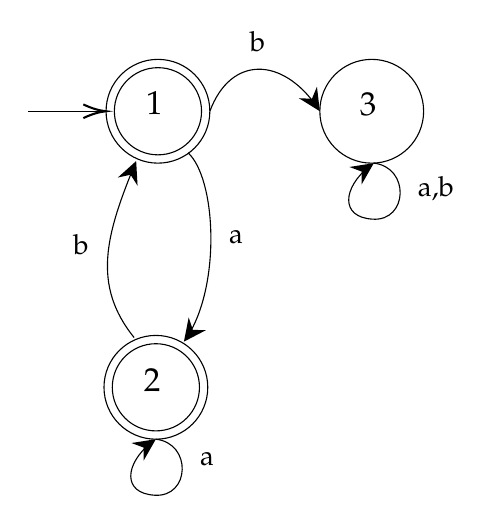
\begin{tikzpicture}[x=0.75pt,y=0.75pt,yscale=-1,xscale=1]
%uncomment if require: \path (0,266); %set diagram left start at 0, and has height of 266

%Shape: Circle [id:dp9412187109416901] 
\draw   (97,64) .. controls (97,50.19) and (108.19,39) .. (122,39) .. controls (135.81,39) and (147,50.19) .. (147,64) .. controls (147,77.81) and (135.81,89) .. (122,89) .. controls (108.19,89) and (97,77.81) .. (97,64) -- cycle ;
%Shape: Circle [id:dp49215165947758543] 
\draw   (101,64) .. controls (101,52.4) and (110.4,43) .. (122,43) .. controls (133.6,43) and (143,52.4) .. (143,64) .. controls (143,75.6) and (133.6,85) .. (122,85) .. controls (110.4,85) and (101,75.6) .. (101,64) -- cycle ;
%Shape: Circle [id:dp34174354582723065] 
\draw   (96,197) .. controls (96,183.19) and (107.19,172) .. (121,172) .. controls (134.81,172) and (146,183.19) .. (146,197) .. controls (146,210.81) and (134.81,222) .. (121,222) .. controls (107.19,222) and (96,210.81) .. (96,197) -- cycle ;
%Shape: Circle [id:dp18662144031095385] 
\draw   (200,64) .. controls (200,50.19) and (211.19,39) .. (225,39) .. controls (238.81,39) and (250,50.19) .. (250,64) .. controls (250,77.81) and (238.81,89) .. (225,89) .. controls (211.19,89) and (200,77.81) .. (200,64) -- cycle ;
%Shape: Circle [id:dp7278735994062155] 
\draw   (100,197) .. controls (100,185.4) and (109.4,176) .. (121,176) .. controls (132.6,176) and (142,185.4) .. (142,197) .. controls (142,208.6) and (132.6,218) .. (121,218) .. controls (109.4,218) and (100,208.6) .. (100,197) -- cycle ;
%Curve Lines [id:da4177480575720798] 
\draw    (136.5,84) .. controls (150.08,96.61) and (152.37,147.8) .. (136.07,172.76) ;
\draw [shift={(134.5,175)}, rotate = 306.87] [fill={rgb, 255:red, 0; green, 0; blue, 0 }  ][line width=0.08]  [draw opacity=0] (10.72,-5.15) -- (0,0) -- (10.72,5.15) -- (7.12,0) -- cycle    ;
%Curve Lines [id:da8880562241813899] 
\draw    (110.5,173) .. controls (90.02,147.65) and (97.12,123.25) .. (110.46,90.53) ;
\draw [shift={(111.5,88)}, rotate = 472.38] [fill={rgb, 255:red, 0; green, 0; blue, 0 }  ][line width=0.08]  [draw opacity=0] (10.72,-5.15) -- (0,0) -- (10.72,5.15) -- (7.12,0) -- cycle    ;
%Curve Lines [id:da8177317836926434] 
\draw    (121,222) .. controls (138.5,224) and (137.5,250) .. (120.5,249) .. controls (104.43,248.06) and (106.23,233.71) .. (118.71,223.7) ;
\draw [shift={(121,222)}, rotate = 505.41] [fill={rgb, 255:red, 0; green, 0; blue, 0 }  ][line width=0.08]  [draw opacity=0] (10.72,-5.15) -- (0,0) -- (10.72,5.15) -- (7.12,0) -- cycle    ;
%Curve Lines [id:da1578527385975219] 
\draw    (226,89) .. controls (243.5,91) and (242.5,117) .. (225.5,116) .. controls (209.44,115.06) and (211.23,100.71) .. (223.71,90.7) ;
\draw [shift={(226,89)}, rotate = 505.41] [fill={rgb, 255:red, 0; green, 0; blue, 0 }  ][line width=0.08]  [draw opacity=0] (10.72,-5.15) -- (0,0) -- (10.72,5.15) -- (7.12,0) -- cycle    ;
%Curve Lines [id:da35588608034649716] 
\draw    (147,64) .. controls (157.19,36.84) and (181.95,37.91) .. (198.49,61.72) ;
\draw [shift={(200,64)}, rotate = 237.6] [fill={rgb, 255:red, 0; green, 0; blue, 0 }  ][line width=0.08]  [draw opacity=0] (10.72,-5.15) -- (0,0) -- (10.72,5.15) -- (7.12,0) -- cycle    ;
%Straight Lines [id:da04416447627779929] 
\draw    (59.5,64) -- (95,64) ;
\draw [shift={(97,64)}, rotate = 180] [color={rgb, 255:red, 0; green, 0; blue, 0 }  ][line width=0.75]    (10.93,-3.29) .. controls (6.95,-1.4) and (3.31,-0.3) .. (0,0) .. controls (3.31,0.3) and (6.95,1.4) .. (10.93,3.29)   ;

% Text Node
\draw (115,53) node [anchor=north west][inner sep=0.75pt]  [font=\large] [align=left] {1};
% Text Node
\draw (114,187) node [anchor=north west][inner sep=0.75pt]  [font=\large] [align=left] {2};
% Text Node
\draw (218,54) node [anchor=north west][inner sep=0.75pt]  [font=\large] [align=left] {3};
% Text Node
\draw (155,120) node [anchor=north west][inner sep=0.75pt]   [align=left] {a};
% Text Node
\draw (80,122) node [anchor=north west][inner sep=0.75pt]   [align=left] {b};
% Text Node
\draw (141,227) node [anchor=north west][inner sep=0.75pt]   [align=left] {a};
% Text Node
\draw (246,94) node [anchor=north west][inner sep=0.75pt]   [align=left] {a,b};
% Text Node
\draw (165,24) node [anchor=north west][inner sep=0.75pt]   [align=left] {b};


\end{tikzpicture}

\begin{prob}\end{prob}

$L(M) = \{ w \in \sigma* | \hspace{5px}  w \hspace{5px} \text{does not start with b and does not contain bb.}\}$


\begin{prob}\end{prob}

\begin{enumerate}[label=(\alph*)]

\item
\begin{tabular}{|c||c|c|}
$\delta$ & 0 & 1 \\

\hline

$q_s$ & $q_s$ & $q_s$ 

\end{tabular}

where $s = q_s$ and $F = \{\}$. $q_s$ represents the starting state,
and there is no final state in this case, because there is no
word that belongs in $\varnothing$.

\vspace{15px}

\item
\begin{tabular}{|c||c|c|}
$\delta$ & 0 & 1 \\

\hline

$q_s$ & $q_e$ & $q_e$

\end{tabular}

where $s = q_s$ and $F = \{q_s\}$. $q_s$ represents the starting state,
and $q_e$ represents a non-empty state. Since we are trying to get to
$\epsilon$, the only acceptable state is the starting state.

\vspace{15px}

\item
\begin{tabular}{|c||c|c|}

$\delta$ & 0 & 1 \\

\hline

$q_s$ & $q_0$ & $q_1$ \\

\hline

$q_0$ & $q_n$ & $q_f$ \\

\hline

$q_1$ & $q_f$ & $q_n$ \\

\hline

$q_n$ & $q_n$ & $q_n$ \\

\hline

$q_f$ & $q_n$ & $q_n$

\end{tabular}

where $s = q_s$ and $F = \{q_f\}$. $q_0$ and $q_1$ represents states in which
the word starts with 0 or 1, respectively. From $q_0$, if a 1 is entered, then we
enter $q_f$, which is the accepting state (similar is true for $q_1$). Any more
letters after that (or if 0 is entered after $q_0$ or 1 after $q_1$), we enter $q_n$, which
is simply a non-accepting state from which we can't exit. 

\vspace{15px}

\item
\begin{tabular}{|c||c|c|}
$\delta$ & 0 & 1 \\

\hline

$q_s$ & $q_0$ & $q_1$ \\

\hline

$q_0$ & $q_0$ & $q_0$ \\

\hline

$q_1$ & $q_n$ & $q_1$ \\

\hline

$q_n$ & $q_n$ & $q_n$
\end{tabular}

where $s = q_s$ and $F = \{q_1\}$. Because we have to start with 1, $q_s$ and $q_n$ 
are here for the situations of $\epsilon$ and when we start with 0, respectively. There is
no exit from $q_n$. Then, for situations we do start with 1, we simply shuffle between $q_1$
and $q_0$, which represents what was the last digit read. 

\vspace{15px}

\item
\begin{tabular}{|c||c|c|}
$\delta$ & 0 & 1 \\

\hline

$q_s$ & $q_0$ & $q_1$ \\

\hline

$q_0$ & $q_n$ & $q_1$ \\

\hline

$q_1$ & $q_0$ & $q_n$ \\

\hline

$q_n$ & $q_n$ & $q_n$
\end{tabular}

where $s = q_s$ and $F = \{q_s, q_0, q_1\}$. Here, the only non-accepting state
is $q_n$, which represents when 00 or 11 has been found. $q_1$ and $q_0$ represents
the last digit read, and simply transitions between each other, except if there is 
a 00 or a 11.

\vspace{15px}

\item
\begin{tabular}{|c||c|c|}
$\delta$ & 0 & 1 \\

\hline

$q_s$ & $q_0$ & $q_1$ \\

\hline

$q_0$ & $q_0$ & $q_1$ \\

\hline

$q_1$ & $q_2$ & $q_0$ \\

\hline

$q_2$ & $q_2$ & $q_1$

\end{tabular}

where $s = q_s$ and $F = \{q_0\}$. The states $q_0, q_1, q_2$ represent the remainder when
the binary string (so far) is divided by three. This logic works because each digit on a binary string
is eventually added together, so whenever the remainder becomes 0, it can be treated as a new string.
For when the remainder is 1, then we can examine 11 or 10 (for the next read). In the prior case, $11_2 = 3$,
so the remainder is 0. In the latter case, $10_2 = 2$, so the remainder is 2. Finally, we can move into
the cases when the remainder is 2. Remainder 2 in binary is 10, so we prepend that to
the next digit and the cases become 101 or 100. The former gives remainder 2 (again), and the latter gives remainder 1.  

\item
\begin{tabular}{|c||c|c|}
$\delta$ & 0 & 1 \\

\hline

$q_0$ & $q_0$ & $q_1$ \\

\hline

$q_1$ & $q_0$ & $q_2$ \\

\hline

$q_2$ & $q_0$ & $q_3$ \\

\hline

$q_3$ & $q_3$ & $q_3$ 
\end{tabular}

where $s = q_0$ and $F = \{q_3\}$. Since the strings $x$ and $y$ can be empty, then this 
simply becomes a search to see if the substring 111 is in this string. $q_0$, $q_1$, $q_2$, $q_3$ 
represents the number of consecutive 1's found, and once 3 are found, $q_3$ doubles as the 
accepting truthy state.

\end{enumerate}

\newpage

\begin{prob}\end{prob}

The code is as follows:
\begin{tcolorbox}
\begin{verbatim}
# Accepts All binary strings in which all two successive ones
# are separated by an odd number of zeroes

start: truthy

accept-states: [truthy]

transitions:
- [truthy, 0, truthy]
- [truthy, 1, open_1]

- [open_1, 0, odd_zero]
- [open_1, 1, falsy]

- [odd_zero, 0, even_zero]
- [odd_zero, 1, truthy]

- [even_zero, 0, odd_zero]
- [even_zero, 1, falsy]

- [falsy, 0, falsy]
- [falsy, 1, falsy]
\end{verbatim}
\end{tcolorbox}

\end{document}
